\clearpage
\section{Modemy v systémech datové komunikace}
\subsection{Jaké jsou základní části modemu? Odůvodněte jejich použití.}
\begin{itemize}
    \item Formátování a zdrojové kódování (pro přizpůsobení zdroje informací pro přenosový kanál)
    \item Skrambler (odstraňuje periodicity)
    \item Protichybové zabezpečení (pro opravu nebo detekci chyb)
    \item Modulace / linkový kód (mění datový signál na signál vhodný k přenosu médiem)
    \item D/A (převod digitálního signálu na analogový)
    \item vidlice (duplex) - přístup na médium
    \item A/D
    \item Demodulace / dekódování
    \item Dekódování protichybového  zabezpečení
    \item Deskrambler
    \item Zpětné formátování a dekódování
\end{itemize}

\subsection{Na jaké základní dvě skupiny dle použitého kmitočtového pásma lze rozdělit měniče
signálu? Vysvětlete pojmy linkový kód, klíčování a modulace, přidružte je výše
dotazovaným skupinám.}
\begin{itemize}
    \item Měniče v základním pásmu (baseband) - využívá linkových kódů, potlačuje stejnosměrnou složku
    \item Měniče v přeneseném pásmu (passband) - využívá se klíčování na nosné, těch může být i více 
    (MultiCarrier modulations)
    \item linkový kód - způsob realizace přenosu v základním pásmu, obdélníkové průběhy, vhodné pro synchronizaci
    \item klíčování - způsob realizace přenosu v přeneseném pásmu, jedná se o digitální modulaci
    \item modulace - přenášení analogového signálu na nosné frekvenci
\end{itemize}

\subsection{Co je to skrambler a k čemu slouží?}
\begin{itemize}
    \item Část modemu převádějící původní signál na pseudonáhodnou sekvenci
    \item Zabraňuje periodicitám, rozkládá výkon rovnoměrně po spektru (výkonová spektrální hustota [dBm/Hz])
    \item Může i šifrovat  data
\end{itemize}

\subsection{K čemu slouží linkové kódy? Jaké jsou základní důvody jejich použití? Uveďte příklady
linkových kódů a technologie, kde se využívají.}
\begin{itemize}
    \item potlačení stejnosměrné složky
    \item zlepšení synchronizace v přijímači
    \item detekce chyb (duobinární linkové kódy)
    \item snížení potřeby šířky pásma (víceúrovňové linkové kódy)
    \item odolnost vůči přepólování u diferenčních linkových kódů (kódují změny mezi bity)
    \item odolnost vůči šumu
    \item Manchester - 10 Mb/s Ethernet
    \item 2B1Q a 4B3T - ISDN rozhraní U
    \item AMI (Alternate Mark Inversion) - ISDN rozhraní S
\end{itemize}

\subsection{Uveďte a popište základní typy klíčování? Uveďte vícestavové klíčovací metody.}
Pozn. \textbf{Skrambler} umožňuje odstranění periodicit a dlouhých sekvencí stejných prvků. Přenos v \textbf{základním pásmu} se realizuje pomocí \textbf{linkových kódů}. Linkové kódování definuje realizace signálových prvků tak, aby byla zejména potlačena stejnosměrná složka.
\begin{itemize}
    \item Při přenosu dat v přeloženém pásmu se používá \textbf{modulační} proces, který nazýváme \textbf{klíčování}
    \item Základní typy klíčování: Amplitudové klíčování (ASK), Fázové klíčování (PSK), Kmitočtové klíčování (FSK).
    \item \textbf{Amplitudové klíčování} lze realizovat pomocí násobičky. Vynásobením nosného signálu datového signálu vznikne amplitudově klíčovaný signál. 
    \item \textbf{Kmitočtové klíčování} lze realizovat přepínáním dvojice oscilátorů nosných signálů s užitím násobičky.
    \item \textbf{PSK} je dvojstavové fázové klíčování. Klíčování je opět realizováno pomocí násobičky, na kterou je přivedena nosná a bipolární datový signál .
\end{itemize}
Čtyřstavové fázové klíčování (QPSK), Osmistavové fázové klíčování (8 - PSK)

\subsection{Vysvětlete princip QAM modulace. O jaký typ klíčování se jedná? Co je to IQ modulátor, zakreslete obrázek. Co je to konstelační diagram? }
\begin{itemize}
    \item V bloku OSMS je datový tok rozdělen na dva o shodné přenosové rychlosti.  Vzniklá dvojice signálů je vstupem IQ modulátoru. Číslice před zkratkou QAM uvádí počet stavů. (Ty se tvoří různými napěťovými úovněmi)
    \item Kvadraturní amplitudová modulace (QAM) reprezentuje vícestavové kombinované ASK-PSK klíčování.
    \item Protože jeden signál je ve fázi (\textbf{I}n phase) a druhý o pí/2 posunut (\textbf{Q}uadrature), označují se tato dvojice jako \textbf{IQ modulátor}.
    
    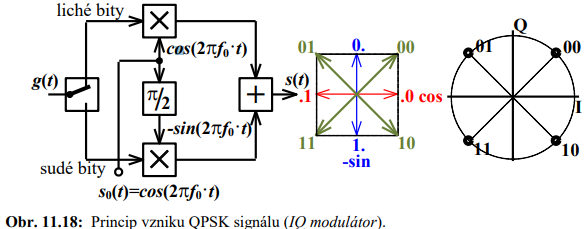
\includegraphics[]{images/image1.png}
    
    \item Fázové klíčování, ale především QAM, se zobrazují s pomocí tzv. \textbf{Konstelačního diagramu}. Diagram uvádí v IQ rovině přiřazení binárních kombinací fázorům nosného signálu.
\end{itemize}

\subsection{Modulace v pojetí protichybového sytému. Co je to eukleidovská vzdálenost? Popište
TCM modulaci?}
\begin{itemize}
    \item Pro lepší rozlišovací schopnosti se nemusejí využít všechny stavy fázového diagramu
    \item Vzniká tak detekční kód
    \item Odolnost udává geometrická vzdálenost mezi stavy (Eukleidovská vzdálenost)
    $d_{Euk}=\sqrt{(x_1-x_2)^2+(y_1-y_2)^2}$
    \item TCM (Trellis Coded Modulation) - Spojení mřížového kódu (stromový kód s konečnou délkou kódového ohraničení)
    a PSK nebo QAM, zavádí stavovou nadbytečnost. Jeden z vstupních proudů je tvořen zabezpečovacími bity.
\end{itemize}
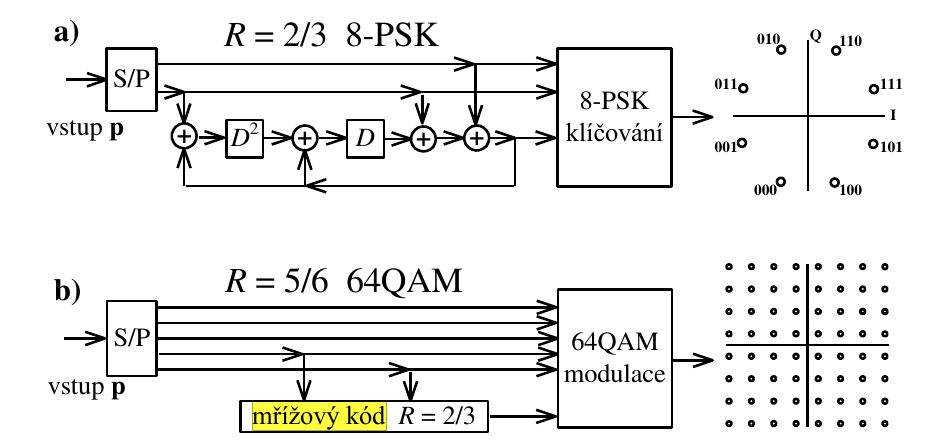
\includegraphics[width=16cm]{images/11_tcm.png}

\subsection{Vysvětlete princip vícetónových modulací DMT/OFDM. Nakreslete obrázek realizace.}
\begin{itemize}
    \item Hledání metod dalšího zefektivnění datového přenosu vedlo k vícetónovým modulačním metodám.
    \item Vstup se dělí do toků, které mají přenosovou rychlost danou počtem bitů na jejich nosných.
    \item Je to několik QAM modulátorů realizovaných pomocí rychlé Fourierovy transformace rozmístěných na spektru
    \item Můžeme se setkat s \textbf{Diskrétní vícetónovou modulací DMT}, která se uplatňuje zejména na telefonních
    přípojkách v ADSL a VDSL, je v základním pásmu, vzniká reálný signál
    \item a \textbf{Ortogonálním kmitočtově děleným multiplexem OFDM}, který se uplatňuje na sdílených médiích
    v technologiích PLC, WLAN, DVB-T, je v přeneseném pásmu, vzniká komplexní signál
    \item  u OFDM jsou komplexní hodnoty vstupem IQ modulátoru, který může být realizován s ohledem na cílové
    kmitočtové pásmo číslicově nebo analogově
    \item Doplní se cyklická předpona
    \item Sériový tok
    \item D/A převod
\end{itemize}
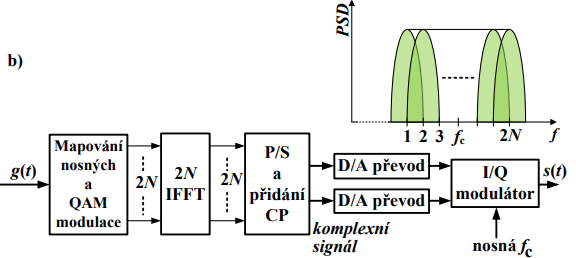
\includegraphics[]{images/11_dmt_odf.png}
    
\subsection{Vysvětlete problematiku korekce přenosových charakteristik. Jaké typy ekvalizérů znáte?}
\begin{itemize}
    \item Zkreslení signálu kanálem
    \item Impulsní charakteristika -> rozšíření znaků -> jejich překrytí (přeslechy mezi symboly)
    \item Může docházet i k přeslechům mezi nosnými
    \item Používají  se ekvalizéry - číslicové filtry
    \begin{itemize}
        \item lineární
        \item DFE (Decision Feedback Equalizer)
        \item TEQ (speciální případ DFE)
    \end{itemize}
\end{itemize}

\subsection{Vysvětlete možnosti realizace duplexního přenosu. Co je to vidlice? Vysvětlete princip
vzniku a potlačení ozvěnového signálu.}
\begin{itemize}
    \item Kmitočtové dělení (jiné směry - jiná pásma, filtr na vstupu i výstupu)
    \item Obvodový duplex s potlačením ozvěnového signálu - obsahuje vidlici, což je obvodový prvek pro oddělení
    \item vidlice - potlačuje ozvěnový signál, aktivní prvek z několika součástí (diferenční zesilovač, vyvažovač,
    sumační zesilovač, invertor)
    \item místní a vzdálená ozvěna - rušení vznikající nehomogenitou a různou délkou vedení, snižuje SNR
    \item ozvěna se potlačuje odečítáním modelového ozvěnového signálu, využívají se číslicové filtry
\end{itemize}
